%%%%%%%%%%%%%%%%%%%%%%% file template.tex %%%%%%%%%%%%%%%%%%%%%%%%%
%
% This is a general template file for the LaTeX package SVJour3
% for Springer journals.          Springer Heidelberg 2010/09/16
%
% Copy it to a new file with a new name and use it as the basis
% for your article. Delete % signs as needed.
%
% This template includes a few options for different layouts and
% content for various journals. Please consult a previous issue of
% your journal as needed.
%
%%%%%%%%%%%%%%%%%%%%%%%%%%%%%%%%%%%%%%%%%%%%%%%%%%%%%%%%%%%%%%%%%%%
%
% First comes an example EPS file -- just ignore it and
% proceed on the \documentclass line
% your LaTeX will extract the file if required
\begin{filecontents*}{example.eps}
%!PS-Adobe-3.0 EPSF-3.0
%%BoundingBox: 19 19 221 221
%%CreationDate: Mon Sep 29 1997
%%Creator: programmed by hand (JK)
%%EndComments
gsave
newpath
  20 20 moveto
  20 220 lineto
  220 220 lineto
  220 20 lineto
closepath
2 setlinewidth
gsave
  .4 setgray fill
grestore
stroke
grestore
\end{filecontents*}
%
\RequirePackage{fix-cm}
%
\documentclass{svjour3}                     % onecolumn (standard format)
%\documentclass[smallcondensed]{svjour3}     % onecolumn (ditto)
%\documentclass[smallextended]{svjour3}       % onecolumn (second format)
%\documentclass[twocolumn]{svjour3}          % twocolumn
%
\smartqed  % flush right qed marks, e.g. at end of proof
%
\usepackage{mhsetup}
\usepackage{amsmath}
\usepackage{mathtools}
\usepackage{natbib}
\usepackage{graphicx}
\usepackage{float}
\usepackage{xyling}
\usepackage[utf8]{inputenc}
\usepackage{gb4e}
\noautomath
\usepackage[T1]{fontenc}
\usepackage{ tipa }
\usepackage{import}
\usepackage{color}
\usepackage{calc}
\usepackage{subfig}
\bibpunct{(}{)}{,}{a}{}{,}
\newcommand{\notejoel}[1]{\noindent \textbf{[[JCW:  #1 ]]}}
\newcommand{\notejoe}[1]{\noindent \textbf{[[JTF:  #1 ]]}}
\renewcommand{\theequation}{\Alph{equation}}

% Insert the name of "your journal" with
\journalname{Journal of }

\begin{document}


\title{Optionality is Stable Variation is Competing Grammars
\thanks{...All errors are the first author's.}}
%\subtitle{Do you have a subtitle?\\ If so, write it here}

%Or, A Unified Theory of Stable and Unstable Variation

%\titlerunning{Short form of title}        % if too long for running head

\author{Josef Fruewald \& Joel C. Wallenberg}

%\authorrunning{Short form of author list} % if too long for running head

\institute{Joel C. Wallenberg \at
              Newcastle University \\
              Tel.: +44-(0)191-222-7366\\
              \email{joel.wallenberg@gmail.com}
}

\date{Received: date / Accepted: date}
% The correct dates will be entered by the editor


\maketitle

\begin{abstract}
stuff
\keywords{syntax \and morphology \and language change \and language acquisition \and evolutionary dynamics}
% \PACS{PACS code1 \and PACS code2 \and more}
% \subclass{MSC code1 \and MSC code2 \and more}
\end{abstract}

\section{Introduction}
\label{intro}

This is a strictly Minimalist proposal, in the sense of \citet{chomsky1993, chomsky1995, chomsky1998,chomsky2001}.
It takes an issue which has frequently been brute-force encoded in the grammar with little explanatory content, namely optionality, and shows how it can be fully explained as an effect of the interface between the narrow grammar (understood here as a maximally simple combinatoric system) and general properties of the linguistic, cognitive, and social systems in which the derivation is produced.
\{Our proposal is also not to postulate a set of \textsl{ad hoc} interface constraints; the phenomenon which appears to be optionality in the phonology and syntax is an interface \textsl{effect}, a by product of how the derivation must relate to independently motivated linguistic and extralinguistic structures.\notejoe{What does this mean?}\}

In this paper, we consider X CASESTUDIES
%six case studies, three syntactic and three (morpho-)phonological, which have been described either as diachronically stable variation or as optional operations: \textsl{-in}/\textsl{-ing} variation, relative clause extraposition, [t]/[d]-deletion, \textsl{h}-dropping, \textsl{whether/if} variation in embedded questions \citep{baileywallenbergwurff2012}, and English topicalization (object DP fronting).
Each case involves a probabilistic (i.e. ``optional'') alternation between surface variants which presumably have the same input to the grammar.
For example, in English TD Deletion, the input to the phonological grammar are words with a final coda cluster, including a coronal stop, and the output is variably simplified.
\begin{exe}
	\ex TD Deletion\\
		\Tree{
		&\K{\it mist}\AR{dl}_{p}\AR{dr}^{(1-p)}\\
		\K{\it mis'} && \K{\it mist}
		}
\end{exe}
%In English and Icelandic {\it whether}/{\it if} variation, the input to the grammar is an embedded question, and {\it if} and {\it whether} are variably selected as exponents of C.\notejoe{In case this is wrong, see alternative below}
%\begin{exe}
%\ex {\it if}/{\it whether} in embedded questions\\
%	 \Tree{
%	&\K{C}\AR{dl}_{p}\AR{dr}^{(1-p)}\\
%	\K{\it if} && \K{\it whether}
%	}
%\end{exe}

In English and Icelandic {\it whether}/{\it if} variation, the input to the grammar is CP projection of an embedded polar question, with either \textsl{whether} or \textsl{Q} having moved to Spec(CP), and {\it if} and {\it whether} are variably pronounced \citep[following][]{larson1985, hanromero2004}. This syntactic structure thus has two possuble spell-outs, with no functional difference in most cases.
\begin{exe}
\ex {\it if}/{\it whether} in embedded questions\\
	\Treek[3]{3}{
		&\K{\fbox{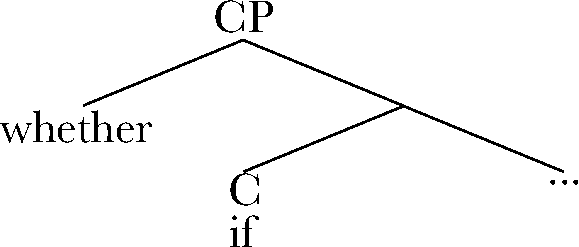
\includegraphics[width = 0.3\textwidth]{figures/whetherif_in.pdf}}}\AR[-4]{dl}_{p}\AR[-4]{dr}^{(1-p)}\\
		\K{\textit{whether}$\rightarrow\emptyset$}
		\Below{\textit{if}$\rightarrow$\textit{if}}&&
		\K{\textit{whether}$\rightarrow$\textit{whether}}
		\Below{\textit{if}$\rightarrow\emptyset$}
	}
\end{exe}


We will argue that these and the rest of our examples are best understood as special cases of ``Competing Grammars'' \citep[][]{kroch1989}.
When a single speaker's inventory of grammatical rules contains multiple rules which have the same structural definition for use, but are mutually incompatible, they could be said to be in competition for use, \textsl{i.e.} to be Competing Grammars.
Grammar competition is typically a diachronically unstable situation, so one rule usually replaces the other.
While Competing Grammars is most often used to explain the dynamics of language change \citep{yang2000,yang2002}, the Minimalist research program demands that we attempt to reduce the explanatory mechanisms for language change and stable variation to just one system.
Our attempt is made easier by the fact that the state of the art in the current  theory of functional heads and movement already predicts that syntactic optionality is the same as competing grammars (i.e. morphosyntactic doublets), though few researchers to date have noticed this \citep[with the exception of][]{kroch1994}.

We argue that stable variation is a special case of Competing Grammars, but the circumstances that give rise to these special cases are not, themselves, grammatical.
Intrinsically unstable grammar competition can become \textsl{almost} diachronically stable under a very specific (and perhaps rare) set of circumstances: when categorical variants have \textbf{partially} specialized along a continuous dimension of use with no clear endpoints (e.g. style, phonological heaviness). 
In this rare case, the interaction between categorical variation and a continuous dimension of use will not allow the construction to fully specialize, though it does allow the potential change in progress to slow to down until it is barely possible to detect. In fact, even then, the specialization does not completely halt the change in progress.
Thus, we are led to the hypothesis that truly diachronically stable variation does not exist.

Figure \ref{competition_figure_first} diagrammatically illustrates the three scenarios of competition between linguistic forms A and B we will investigate, provided here to frame the discussion. 
The first, and most common scenario, involves the introduction of a new variant B into speakers' grammatical ruleset.
Speakers may variably use both A and B for a period of time, but eventually use of B becomes categorical and A is eliminated.
The second possible scenario is that variant B enters speakers' grammatical ruleset, and again, speakers may variably use both A and B for a period of time.
In this scenario, however, A and B fully specialize for use in different contexts, and no longer compete for use within these contexts.
For example, A could take on a more specialized meaning, like {\it luncheon} did after the introduction into usage of the truncated form {\it lunch}.
The final scenario, the primary subject of our discussion, is the {\it partial} specialization of A and B along a continuous dimension, like sociolinguistic style.


\begin{figure}[h!tbp]
	\centering
	\subfloat[][Replacement]{
	 	\def\svgscale{0.55}
		\import{figures/}{replacement.pdf_tex}
		\label{replacement_first}
	}
	\qquad
	\subfloat[][Specialization]{
		\def\svgscale{0.55}
		\import{figures/}{specialization.pdf_tex}
		\label{specialization_first}
	}
	\qquad
	\subfloat[][Partial Specialization]{
		\def\svgscale{0.55}
		\import{figures/}{partial_specialization.pdf_tex}
		\label{partial_specialization_first}
	}
 \caption{The possible outcomes of competition. Outcome (c), partial specialization, represents apparent stable variation.}
 \label{competition_figure_first}
\end{figure}


  
In the first section below, we introduce the problem of stable variation in the sociolinguistic and phonological literature, and show how it relates to syntactic optionality.
In particular, we show how optionality in syntax can only be described in a Minimalist framework as doublets of functional heads, which is really the same as Competing Grammars.
%, and that this poses a problem for language acquisition. \notejoe{acquisition all of a sudden}
In section \S\ref{solution}, we show that stable variation can persist just in case the variants become specialized in use along a particular type of continuous dimension.
Section \S\ref{cases} presents our case studies, and shows how they are all situations in which variants have become semi-specialized along a continuous dimension of use, which is the only circumstance that could allow such variation to persist indefinitely.
Lastly, we conclude and offer some predictions that this approach makes for future research.


Before continuing, we should be clear that there are some well defined problems in the study of language change, chief among them being the Actuation Problem, originally framed by \citet{wlh1968} as the following question:
	\begin{quote}
		Why do changes in a structural feature take place in a particular language at a given time, but not in other languages with the same feature, or in the same language at other times? This \textsl{actuation problem} can be regarded as the very heart of the matter.
	\end{quote}
Since 1968, the Actuation Problem has remained both a problem and close to the very heart of the matter of language variation and change.
Addressing the Actuation Problem is well beyond what we will be able to do in this paper.
So, for example, the means by which a variant B in Figure \ref{competition_figure_first} is introduced is completely unspecified.
However, we don't believe that lacking even an adequate theory of actuation poses a problem for the models we outline here, since they mostly involve dynamics of the language system well after the actuation of changes.

\section{The Problem of Stable Variation}
\subsection{Optionality in Minimalism}

An important unification of different aspects of language change was presented in \citet{kroch1994}.
\citet{kroch1994} showed that syntactic variation and change can be viewed as the same phenomenon as morphological variation and change, i.e. morphological doublets where morphological features are spelled out in two alternative ways, such as \textsl{dived}/\textsl{dove}.
Kroch presents his view of the ``Blocking Effect'' (originally stated by \citealt{aronoff1976}; see also references in \citealt{kroch1994}), which he explains as a diachronic pressure for morphological doublets to disappear over time.
Though any individual can learn synonyms or alternate spell-outs for the same morphological features, the alternatives do not stably coexist over long periods of time.
Rather, one alternative replaces the other, or the two alternatives specialize in some way so that they no longer overlap in use.
This specialization can be the reanalysis of one variant as spelling out a different set of morphological features, but it does not need to be reanalyzed in that very specific sense: as long as the variants become restricted to non-overlapping contexts, they no longer ``block'' each other, i.e. compete for use.

One key insight of \citet{kroch1994} is that in a Minimalist syntactic system, the Blocking Effect of diachronic morphology (or synonyms generally) applies straightforwardly to the syntax as well.
In Minimalism, the syntax is a highly generalized process of combining and projecting syntactic heads.
Thus, syntactic parameters (e.g. word order) must be the exponents of features on the syntactic heads, which then show themselves as these heads combine with complements and project, etc.
In this way, variation between two word orders such as OV and VO is really the same as a morphological doublet: the ``competing grammars'' \citep{kroch1989} are just alternative featural versions of a single syntactic head, e.g. $v$, and whichever version is used in a given sentence leads to certain effects on the rest of the structure and the resulting string.
The diachronic instability of having multiple versions of the same basic head is then just the Blocking Effect from morphology, and needs no additional statement in a theory of language change: there is a pressure against different exponents for the same meaning and function, because they ``block'' each other by competing for use, both being alternative possibilities in a particular context.
Just as in morphology, one syntactic variant will replace the other, unless the two versions of the relevant head somehow specialize such that they no longer overlap in use (and Kroch gives some examples where this seems to have occurred in the syntactic domain).

In a Minimalist syntax, the trigger for any movement can only be the featural content of some functional head \citep{chomsky2000, chomsky2001}, and ``optional'' movement is the result of different flavors of the same functional head being selected.
For example, take the following example of topicalization.
\begin{exe}
\ex \label{princetop2_first} She was here two years.
[checking transcript] Five semesters she was here.\\
\citep[][8,9]{prince1999}
\end{exe}
While the topicalization of ``five semesters'' was felicitous, it was not obligatory, as can be seen in the modified version in (\ref{princeuntop2}).
\begin{exe}
\ex \label{princeuntop2} She was here two years.
[checking transcript] She was here five semesters.\\
\citep[Adapted from][8,9]{prince1999}
\end{exe}
For simplicity's sake, we will describe the construction as fronting to Spec, C (the standard assumption prior to \citealt{rizzi1997}), though the exact position targeted by the movement is not relevant to the question at hand.
In (\ref{princetop2_first}), the DP ``five semesters'' was fronted to Spec, C due to the features on C.
We might call this flavor C$^{Top}$.
In (\ref{princeuntop2}), ``five semesters'' remained \textsl{in situ} because a different flavor of C (we might call it C$^{plain}$) was selected, which did not trigger the raising of the DP.

There is no \emph{formal} distinction between the situation with C, where there are two possible flavors of C which produce (non)topicalization in (\ref{princetop2_first}) and (\ref{princeuntop2}), and the competing flavors of $v$ which were involved in an OV to VO word order change.
The only difference is that in the former case, both flavors of C remain in use by speakers for an extended period of time, while in the latter, one flavor of $v$ replaced the other in use entirely.
We believe this difference is due to processes of sociolinguistic history which we will try to elucidate throughout the rest of this paper, not due to processes in the narrow grammar.
Therefore, we are advocating a reimagining of optional linguistic processes: all ``optional'' syntactic operations must also be instances of competing grammars (i.e. morphosyntactic doublets), and vice-versa.

\subsubsection{More on syntactic optionality}
Since we are springing off from the formal identity of Competing Grammars and optionality, let's first justify the approach to treating optionality as being due to different flavors of functional heads.

A maximally simple syntactic system has a great deal of predictive power because of its inherent rigidity, and such a theory accordingly does not leave many possible analyses of an optional movement phenomenon.
A Minimalist syntax does not allow for any construction-specific transformational rules, only one generalized transformation for putting syntactic pieces together: Merge (with Move being subtype of Merge, either combined with Agree, as in \citealt{chomsky2000}, or not, as in \citealt{chomsky2004, chomsky2008}).
When a head, H, has projected once (H'), it can combine with a specifier and project again either by Merge (external) or Move.
What determines whether Merge or Move is used, or indeed, whether the head projects again at all, is whether the head has a feature which must be checked against a particular type of XP in a spec-head configuration.
So far so good, for obligatory movements.
If a certain feature $F$ motivates movement, and H has that feature (H$^F$), then the movement occurs; otherwise (H$^\emptyset$), the movement does not.
Because the default in a maximally simple (i.e. Minimalist) system is no movement at all, there is simply no way to encode optional movement with a feature.
(Note that ``Merge...preempts Move'' requires no movement to be a default in the system, as initially pointed out in \citealt{chomsky2000}.)

The only way to state an optional movement in such a syntactic system, without adding new theoretical machinery, is by allowing the speaker's inventory of functional heads to include two flavors of the same functional head H, one with the movement-triggering feature: H$^F$ and one without H$^\emptyset$.
The speaker can then choose to form a numeration with either H$^F$ or H$^\emptyset$.
This is a morphosyntactic doublet, by definition, of the same type discussed in Kroch (1994): two formal variants with no difference in narrow meaning and overlapping discourse environment.
This is simply the definition of ``competing grammars'' \citep{kroch1994}, as the variants are inherently in competition for use in a particular discourse context.
One could certainly imagine adding new mechanics to the syntax to encode optionality directly (thus fundamentally rejecting the basic proposals of a Bare Phrase Structure \citep{chomsky1995} and most Minimalist syntax), and the literature is full of proposals such as: getting around the idea that no movement is a default, adding some kind of stochasticity to the features on heads themselves (H$^{[pF]}$ where $p$ is some probabilty)\notejoe{Joel, look at this parenthetical}, or adding a whole post-processing system consisting of probabilistic trans-derivational filters \notejoel{maybe cite someone for these}.
However, the simple Minimalist system is interesting precisely because it restricts our analytical possibilities and makes certain predictions as a result, so perhaps we should pursue this particular consequence of the system before complicating it.

%%Todo: possibly rewrite top part bc of repeated top examples
Let's revisit the English topicalization construction, as shown in the final sentences of (\ref{princetop2_first}) above (repeated as \ref{princetop2} below) and (\ref{princetop1}).

\begin{exe}
\ex \label{princetop1} She's going to use three groups of mice.
One, she'll feed them mouse chow, just the regular stuff they make for
mice.
Another she'll feed them veggies.
And the third she'll feed junk food.\\

\ex \label{princetop2} She was here two years.
[checking transcript] Five semesters she was here.\\
\citep[both examples from][8,9]{prince1999} 

\end{exe}

\noindent As was well-known even in the early days of generative syntax, English allows objects (and other XPs) to be fronted to a specifier position in the high left-periphery in certain discourse contexts.
\citet{prince1985,prince1998, prince1999} shows that this fronting is felicitous in two English discourse contexts, both of which require a certain type of contrast to appear on the fronted XP, though one context involves a backgrounded (i.e. topical, assumed) XP and the other an XP with information-structural focus (a distinct notion to contrast); these two contexts are shown in (\ref{princetop1}) and (\ref{princetop2}), respectively.

However, even in these two contexts where topicalization is felicitous, it is never obligatory.
Leaving the XP \textsl{in situ} is equally felicitous, provided that the same accent pattern is maintained.
Thus, as long as the XP that was fronted in sentences (\ref{princetop1}) and (\ref{princetop2}) is still accented, and as long as \textsl{junk food} in (\ref{untop1}) is also accented, the same sentences without the fronting can be used in the same discourse context, as shown in (\ref{untop1}) and (\ref{untop2}).\footnote{Perhaps the required prosody is somewhat more awkward with this word order, leaving the object \textsl{in situ}.
Similarly, the \textsl{in situ} versions of (\ref{dem1}) and (\ref{dem2}) definitely require a different prosody from the fronted versions shown below.
These are both important points, and we return to the prosodic issue in section \ref{topsect} below.} 

\begin{exe}
\ex \label{untop1} She's going to use three groups of mice.
One, she'll feed them mouse chow, just the regular stuff they make for
mice.
Another she'll feed them veggies.
And she'll feed the third junk food.\\

\ex \label{untop2} She was here two years.
[checking transcript] she was here five semesters.\\
\citep[Adapted from][8,9]{prince1999}
\end{exe}


To these two versions of this construction, \citet{caitldiss} adds a third context which involves a demonstrative being fronted, as shown in the two sentences below.


\begin{exe}
\ex \label{dem1} I promised that, if you voted in favour, I would respectfully ask UCU's forthcoming Congress to agree the changes.
This I will now do.\\
(UCU General Secretary, Sally Hunt)
\ex \label{dem2} I would do the following experiment.
This, only some people seem to be able to see,... and others not.\\
(Richard Feynman, Lecture on Color Vision, Caltech, March 6, 1962)
\end{exe}

\noindent \citet{caitldiss} argues extensively that even though these examples do not show the same type of contrast (or the same accent) on the fronted object as (\ref{princetop1}) and (\ref{princetop2}), the demonstrative itself is inherently contrastive, and this licenses the fronting construction.
Again, the sentences would be perfectly felicitous in context if the demonstrative were not fronted, and the meaning is apparently unchanged.
Thus, the fronting is truly optional.

Keeping the syntactic system as simple as possible, the movement to Spec, C must be triggered by some feature on C which attracts an XP to value its feature.
For simplicity's sake, we will follow \citet{caitldiss} and assume that some notion of contrast (though a subtle one) defines the set of XPs which could be fronted in the English topicalization construction, and these XPs bear a feature like [constrast].
When the fronting occurs, it is because there is a version of C in the phrase structure which probes for an XP bearing the feature [contrast].
In that case, C$^{[u~\text{contrast}]}$ must attract the XP to its specifier.
In the situation where the fronting does not occur, this is only possible if a different version of C is used which is not a Probe for [contrast].
Thus, there are two versions of C in the speaker's inventory of functional heads: \{C$^{[u~\text{contrast}]}$, C$^\emptyset$\}, and the construction is the result of the speaker choosing a particular version to include in the numeration.
This is by definition a morphosyntactic doublet: two heads which differ only in formal syntactic features, and which overlap in use (both in their position in the structure and in this particular information-structural context).\footnote{Note that my basic argument is unaffected if one assumes that topicalization is the result of an ``edge feature'' (EF) on C, as suggested in \citet[][151]{chomsky2008}.
There would still have to be two versions of C, one with the EF, and one without the EF (or equivalent).
Though \citet{chomsky2008} does not deal with this explicitly, if topicalization were due to an EF, there would still need to be some mechanism for specifying the version of C that is used when no type of fronting to Spec, C takes place at all.}
At this point the following question arises: if topicalization vs. no topicalization is a case of competing grammars, then why has it persisted in languages such as English for so long, and why does the phenomenon still persist?
Surely, according to \citet{kroch1994} and the Blocking Effect, one version of C should beat out the other one over time.
The rest of this article addresses the various factors that determine this outcome, and how replacement of one variant by another can be stopped or slowed.
We will return to the specific case of topicalization briefly in section \ref{topsect}.

\subsubsection{Summing up optionality and competing grammars}
Let's assume that syntactic change involves functional-head variants competing for use in a given utterance.
These competing grammars, or morphological doublets, are a kind of partial bidialectalism, at least at the level of the speaker's inventory of functional heads.
If optional syntactic processes can only be described as functional-head variants competing for use, then all optional syntactic processes would also be a form of partial bidialectalism.
This may seem like a difficult idea to swallow, probably only because it offends our naive intuitions about our own linguistic competence.
But since intuiting how the brain works is notoriously unreliable for any brain-process that has been studied, and our idea is certainly no more counterintuitive than the rather baroque organization of the mammalian visual system (both in the eye and in the brain), we suggest that it is worthwhile to suspend disbelief and see if the competing grammars analysis of optionality makes any interesting predictions.
Theoretically, it is certainly a nice result, since we no longer need different machinery to account for change over time and synchronic optionality.


One prediction is immediately clear and, we hope, testable: \citet{kroch1989,kroch1994} states that the morphosyntactic doublet situation is inherently unstable over time.
Either the members of the doublet specialize in use, or the doublet resolves with one member taking over the entire function and causing the other member to drop out of use entirely.
It follows that optional syntactic processes are also inherently unstable over time, and one of these two outcomes should hold for the two syntactic options.
How then can anything like an optional syntactic movement (or an optional phonological rule, for that matter) exist for a long period of time? This is the question which the rest of the article addresses.
We suggest that no variable linguistic process can truly exist stably over time; in all cases of categorical variation, one variant must win out eventually, unless the variants undergo a process of specialization for different environments, meanings, or functions.
However, it is possible for some categorical linguistic processes (or doublets) to remain stochastic (i.e. optional) in their behavior over long periods of time at a \textsl{nearly} stable frequency of application without fully specializing. 


%%%%What about using t-glottaling??? as an example%%%%

\subsection{Expanding the Argument to Phonology}

It may not be immediately obvious how an argument based on competing flavors of functional heads in a Minimalist grammar can be carried over into phonology, but this may have more to do with prevailing theoretical trends obscuring the empirical similarities across these domains.
\citet*{fruehwaldgresswallenberg2013} identified a major point of similarity between syntactic and phonological change: that they exhibit the same quantitative profile, the Constant Rate Effect \citep{kroch1989}.
There was no {\it a priori} reason that both syntactic and phonological change should exhibit the Constant Rate Effect, but in fact, they do.
In the interest of pursuing the question of how far these similarities go, and of developing a general formal theory of optionality, we will be extending the same arguments from syntactic optionality to phonological optionality.





However, we will not be able to be as similarly explicit in the formulation of of the phonological model as we have been in the syntactic model, largely because, as we just said, prevailing theoretical trends do not easily submit to a Competing Grammars analysis of phonological variation.
There are at least three trends which make a Competing Grammars analysis of phonological variation non-trivial.
\begin{exe}
	\ex \label{ot-tend}
		 The popularity of free-generate-and-filter phonological grammars, like Optimality Theory, its descendants and predecessors.
	\ex \label{gram-tend}
		The tendency to account for the conditioning factors in variation by additional grammatical principles in the narrow grammar.
	\ex \label{prob-tend}
		The tendency to incorporate probabilities into the narrow grammar.
\end{exe}


Free-generate-and-filter grammars make it difficult to localize optionality in the way necessary formulate a competing grammars analysis because it isn't possible localize variation to a single to parameter of the grammar in a simple way.
For example, \citet{Coetzee2012} propose the following constraint set to a Noisy Harmonic Grammar to account for contextual conditioning on English {\it t/d} Deletion.
%% How do we align tables to the top of the example number?
\begin{exe}
	\ex \label{noisy.hg}\  \\
\begin{tabular}{lp{3in}}
	*{\sc Ct}]$_{Word}$& Assign one violation mark for every word that ends in the sequence [-Ct] or [-Cd]\\
	{\sc Max} & Assign one violation mark for every input segment lacking an output correspondent (no deletion).\\
	{\sc Max-Pre-V} & Assign one violation mark for each segment that appears in pre-vocalic context in the input, and that does not have a correspondent in the output (no deletion before a vowel).\\
	{\sc Max-Pre-Pause} &Assign one violation mark for each segment that ap- pears in pre-pausal context in the input, and that does not have a correspondent in the output (no deletion be- fore a pause).
\end{tabular}
\end{exe}
In classic Optimality Theory, these constraints lead to a set of 5 different crucial rankings, or competing grammars, in order to account for just two output variants.
In fact, it is the case that if the OT analysis of any given variation involves more than one crucial ranking between two constraints (and they almost always will), there will be more grammars than there are output variants.
In order to adhere to both a Competing Grammars analysis and an OT grammar, we would have to stipulate first that all optionality is the result of variation in just one crucial ranking, a theoretical challenge to be sure.

The tendency to account for conditioning of variation with additional grammatical principles, and the incorporation of probabilities directly into the narrow grammar are two closely related theoretical tendencies which obscure similarities between phonological and syntactic variation.
Take, for example, the finely articulated specification of a variable rule from \citet{3288} for {\sl t}/{\sl d} Deletion in African American English.
\begin{exe}
 \ex $\left[\begin{array}{rl}
	-&\mbox{cont}\\
	-&\mbox{grav}\\
	-&\mbox{nas}\\
	-&\mbox{comp}
\end{array}\right] \rightarrow (\emptyset) / 
\left[
	\begin{array}{rl}
		\alpha & \mbox{cons}\\
		\zeta &  \mbox{obstr}
	\end{array}
\right]\gamma(\mbox{+})\delta(\mbox{+})
\left[
	\begin{array}{l}
	\underline{\hskip 35pt}\\
	\epsilon~\mbox{voice}
	\end{array}
\right]
\beta(\sim \mbox{V})$ \label{variable.rule}
\end{exe}

The variables, $\alpha, \beta, \gamma \ldots$ included in the definition of the triggering environment represent weights, or preferences, which bias the application of the deletion process. 
They are assigned in order of the magnitude of the effect ($\alpha$: whether or not the preceding segment is consonantal\footnote{From the data in \citet{3288}, it appears that in AAE, {\sl t}/{\sl d} deletion is not absolutely restricted to occur only within coda clusters.
Rather, it is just more likely to occur in coda clusters.
This raises an interesting question as to which elements ought to be included in the categorical vs.\ probabilistic components of variable descriptions.},
$\beta$: whether or not the following segment is a vowel), and are attached to features of segmental phonology (including those of the target) and to morphological boundaries (the $\gamma$ and $\delta$ effects).
\citet{Coetzee2011} offer a nice summary of more recent approaches to incorporating variation into grammars within different flavors of Optimality Theory, including Partially Ordered Constraints (essentially a form of underspecification, similar to the approach by \citet{adger2006} to morphosyntactic variation), Stochastic OT, Noisy Harmonic Grammars, and Maximum Entropy Grammars.
These formalisms differ in their evaluation, and in the probability distributions they produce, but one qualitative similarity between them is that they all encode the conditioning of variation \emph{within the grammar}, thus explicitly conflating stochastic patterns of \textsl{language use} with the generative apparatus that is responsible for phonological derivations.
For example, looking back at the constraints from \citet{Coetzee2012}, {\sc Max-Pre-V} and {\sc Max-Pre-Pause} are additional grammatical principles introduced in order to account for the lower rate of {\sl t}/{\sl d}-deletion before vowels and pauses.
The fact that {\sl t}/{\sl d}-deletion occurs less often in these contexts is an observed pattern in language use, but the question we're putting forward is whether this should be also treated as a \emph{grammatical} fact.

The Competing Grammars approach to variation is fundamentally different from the probabilistic grammar approach in the following way: the factors which influence the selection of one grammar or the other are not themselves part of the grammar; they are influences on \textsl{language use}.
Redescribing the constraint set in (\ref{noisy.hg}) in terms of Competing Grammars would give us the constraint set in (\ref{competing.ot}), which eliminates the contextual versions of {\sc Max}.
The two competing grammars given this constraint set are given in (\ref{ot.grammars}).
Grammar 1 (\ref{ot.grammar1}) produces {\sl t}/{\sl d} deletion, and Grammar 2 (\ref{ot.grammar2}) does not.
\begin{exe}
	\ex \label{competing.ot}\ \\
	\begin{tabular}{lp{3in}}
	*{\sc Ct}]$_{Word}$& Assign one violation mark for every word that ends in the sequence [-Ct] or [-Cd]\\
	{\sc Max} & Assign one violation mark for every input segment lacking an output correspondent (no deletion).
	\end{tabular}
	\ex \label{ot.grammars}
		\begin{xlist}
			\ex Grammar 1: *{\sc Ct}]$_{Word}$ $\gg$ {\sc Max} \label{ot.grammar1}
			\ex Grammar 2: {\sc Max} $\gg$ *{\sc Ct}]$_{Word}$ \label{ot.grammar2}
		\end{xlist}
\end{exe}

The selection of Grammar 1 or Grammar 2 is probabilistic, and driven, we suggest, by the same kind of cognitive system that selects different flavors of functional heads in syntactic variation, or even different lexical synonyms.
It has been richly established that Topicalization and Heavy NP Shift are sensitive to syntactic and pragmatic factors, as well as prosodic factors, such as the phonological weight of the XP to be moved \citep[e.g.][]{arnoldetal2000, speyer2008, speyer2010, wallenberg2015}. %% Citation Please
Likewise {\sl t}/{\sl d} deletion is sensitive the featural properties of the preceding and following segments, morphological boundaries, frequency of the target word, and as recently demonstrated by \citet{MacKenzie.Tamminga2012, tamminga2014}, whether or not {\sl t}/{\sl d} deletion applied at its most recently preceding opportunity. 
It has also been richly demonstrated that speakers utilize all kinds of non-linguistic information in the process of speech perception, including perceived age and social class of the speaker \citep{Hay2006}, and the speaker's race \citep{StaumCasasanto2010}, all properties which would probably be best left out of the narrow grammar by a reasonably conservative theory.
The proposal of the Competing Grammars hypothesis is that all of these influencing factors exist outside of the grammar proper.

It is worth noting explicitly that while we feel it valuable to move most of these influencing factors out of the narrow grammar, that does \emph{not} mean that we want to move them out of the study of linguistics. Just because conditioning factors might not be part of the narrow grammar does not mean that speakers don't have systematic knowledge of them, nor is it the case that linguistic theory ought to be synonymous with the study of narrow grammar.
 
Is it worthwhile to try to reframe phonological variation in terms of Grammar Competition?
Obviously, our answer is yes.
First, from a purely conceptual perspective, it is desirable to reduce the number of entities and phenomena proposed by a theory.
By recasting phonological variation in terms of Competing Grammars, we are bringing the phenomena of syntactic and phonological variation under the same explanatory principles, and therefore subject to the same analytical tools.
Note that it is not necessary that we posit the same or even similar formal systems for the syntactic and phonological grammars themselves; just that there is a unitary mechanism for linguistic variation: the cognitive systems which govern language use can make a selection from among syntactic grammars and phonological grammars in a similar way.


%\notejoel{Talk about specialization of them/'em and it/hit}
%Describe that we are generalising PoC to linguistic structures of an arbitrary type and linguistically important dimensions of an arbitrary type. Which should be done, if it is really a learning strategy. And the same problem with learning if you dont have this for word learning, the same problems apply to structure learning. 

\section{Solution}
\label{solution}

\subsection{Principle of Contrast: Why does specialization occur?}

Beginning with \citet{clark1987} (and subsequent work; e.g. \citealt{clark1990}), we see a plausible explanation for the existence of the Blocking Effect which Kroch used to explain the instability of morphological doublets.
It is the result of a strategy used by children during first language acquisition, the ``Principle of Contrast''.
Clark proposes that children during acquisition assume, wherever possible, that contrasting word forms have contrasting meanings.
Of course, it is possible for children to acquire synonyms, but Clark provides evidence that this is never the first hypothesis when a child is acquiring two phonologically distinct word forms.
If we extend the Principle of Contrast beyond simple words to functional heads, then we can derive the morphosyntactic Blocking Effect of \citet{kroch1994} from an independently motivated constraint on acquisition.
This is not to say that doublets cannot be learned by a given child, of course; it means that children try to distinguish 2 forms in use if at all possible as an acquisition strategy, which can lead to the specialization of two variants for different functions over time.
Doublets specialize over time because generations of children repeatedly try out hypotheses which specialize the forms for different uses.

How, exactly, a speech community will strike upon the same theory of specialization for a competing doublet is an open question.
Presumably, individual learners will initially arrive at idiosyncratic hypotheses, then through processes coordination \notejoe{Clark game theory stuff?} and cultural evolution \citep{kirby.cornish.smith2008} the speech community will converge. 
There are a number of examples of this kind of process clearly taking place in lexical competition.
For example, \textsl{shirt} and \textsl{skirt} have the same etymological source with the latter being borrowed into English from Old Norse \textsl{skyrta} (``shirt'', to the extent that the garment type can be deduced; \citealt{cleasbyvigfusson}).
They were likely to have been synonymous or nearly synonymous, as far as we can tell based on their shared etymology and overlapping meanings in Middle English (cf. e.g. citations in the \textsl{OED}).
However, the two terms clearly specialized over time along two binary dimensions (not exactly simultaneously): upper garment vs. lower garment, male garment vs. female garment.
Both are obvious categorizations of clothing in human society, but neither was, to our knowledge, a component of the original meaning of the words.
A more contemporary example is variation in the terms \textsl{cougar, mountain lion, puma}, and for some speakers, \textsl{panther} and \textsl{catamount}, for the species \textsl{puma concolor}.
While few speakers would call the same animal by all of these names, and some are region-specific, many speakers have 2-3 terms for the same feline.
And while speakers may have some intuition that the terms refer to different cats in some way, they may have so poor a sense of the difference that they cannot report any difference at all (as is the case for one of the authors of this article).
Until some of the terms drop out of use entirely in a particular speech community, different speakers may posit different interpretations, but the interpretations can differ (by chance) along so many possible dimensions of cat characteristics that a consensus is unlikely to develop in the speech community.
Ultimately we would expect a situation like this one to resolve with some of the terms dropping out of use, if any of the terms have any sort of evolutionary advantage over the others (e.g. if one were less marked phonologically).
However, their metaphorical uses referring to women have specialized fairly strictly in the US: \textsl{cougar} for a woman over c. 40 years old dating a man in his twenties or late teens, and \textsl{puma} for a younger woman (e.g. 30s) dating a man in his twenties or late teens.

Just like the Principle of Contrast pushes competing lexical items to specialize in meaning, we posit that it pushes competing functional heads and grammatical rules to similarly specialize.
As the examples of lexical competition (\textsl{shirt}$\sim$\textsl{skirt}, \textsl{cougar}$\sim$\textsl{puma}) demonstrate, the possible dimensions along which competing doublets can specialize are rich and can be culturally specific.
Barring theoretical breakthroughs in cultural anthropology, a comprehensive model of the dimensions along which competing doublets can compete will not be forthcoming.
Sufficed to say, they may be purely linguistic (e.g. constituent heaviness, polarity of embedded questions), purely social (e.g. language choice in a bilingual setting \notejoe{ok a ref for this}), or a mixture of the two.
The key feature of the dimension of specialization is whether it is \emph{categorizable}, or \emph{continuous}.
Specialization along categorizable dimensions will be more likely to completely specialize (e.g. \textsl{shirt} and \textsl{shirt}).
Specialization along continuous dimensions will lead to only partial specialization (e.g. constituent weight and topicalization).


 \subsection{How variants specialize}
 \label{options}
%First, we assume that in cases of stable variation, there is no selective pressure, in the sense of Darwinian selection. If there were some selective pressure in favor of a certain variant, then one variant would replace the other and the problem of the doublet would resolve in that way.
%If there is no such selective pressure favoring one of the variants, then that only leaves the relatively weak pressure of the Principle of Contrast in acquisition.  
%Think about if the above is really necessary as far as no selection. Could it be that Principle of Contrast can supersede selection? This is just like an evolutionary stable stratey, competing for use.
Once a morphosyntactic, lexical, or phonological doublet develops, whether through language contact or some internal development, it becomes an acquisition problem by virtue of the Principle of Contrast. 
However, as \citet{kroch1994} and \citet{yang2000,yang2002} are at pains to point out, this does not mean that children fail to acquire both members of the doublet; speakers can learn doublets, leading to intraspeaker variation.
Rather, following Clark (1990) and the experimental work cited therein (e.g. \citealt{markmanwachtel1988}), we assume that once children have learned the doublet, they will try to distinguish the members of a doublet for different uses, even in the absence of any clear data showing them that the forms have different meanings or different distributions in terms of linguistic or social contexts. 
In the simplest case, this results in a partial mapping of discrete linguistic forms on to discrete dimensions, such as some of the simpler categories of meaning we mentioned above, or something like particular morphosyntactic or phonological contexts. 
Over time (and generations), the linguistic forms will increasingly come to be associated with the discrete categories of use, until the forms are finally completely specialized and they no longer overlap in use at all. At that point, the doublet has fully resolved and no further change is predicted.
%This is the case of categorical variation being specialized along a categorical dimension of specialization, which ultimately leads to complete specialization over time and no more competition (as long as one variant doesn't compete the other out of existence before the specialization has a chance to progress sufficiently).
We can call this the case of \textsl{complete} specialization.

However, if the two (or more) discrete linguistic variants are mapped on to a continuous dimension of use that does not have clear endpoints, then the mapping can never be complete and the forms will always overlap in use to some extent.
This is \textsl{partial} specialization: because there is a mismatch between the mathematical properties of the doublet (it is categorical) and the domain of specialization which speakers have decided is the most salient (it is continuous), it is impossible for either variant of the doublet to be reserved wholly for a single, clear context.
Thus, stochastic production of both variants will continue indefinitely in all contexts with the probability of producing one variant or the other will being affected continuous domain of specialization.
We propose that when this occurs, the change will still stop at some point (i.e. the Principle of Contrast is satisfied and specialization ceases).
In such a case, the Principle of Contrast may succeed in removing most of the competition between the two variants, but they will still overlap in use to some extent because it is simply impossible to map them onto the relevant continuous dimension of specialization such that they no longer compete at all.
Thus, although the competition should in principle resolve itself, it only resolves enough to slow down the change in progress: it will never fully resolve as long as the linguistic variants continue to be associated with the continuous dimension.
The specialization can also never completely stop the change in progress in this case, either, though it can slow the change down until it is virtually indistinguishable from diachronic stability (with drift) when observed within certain windows of time.
We will consider such a case in section \ref{relclause} below.

Thus, our theory of variation predicts that every observed case of synchronic optionality/variation is in fact one of the following three scenarios, which were introduced diagrammatically in Figure \ref{competition_figure_first}:

\begin{exe}
	\ex \begin{xlist}
		\ex A replacement change in progress (outright competition going to completion).
		\ex A replacement change that was arrested due to complete specialization (elimination of competition).
		\ex A replacement change that was slowed due to partial specialization along a continuous dimension (partial elimination of competition).
	\end{xlist}
\end{exe}



\subsection{Example: Whether/If in Historical English and Icelandic}
\label{whetherifsect}

A quantitative study of embedded polar questions in English and Icelandic shows that the same doublet can resolve by \textbf{complete specialization} in one language or speech community, but by \textbf{replacement} in another. Bailey, Wallenberg, \& van der Wurff (2012) and \notejoel{add recent ref} compared the use of \textsl{whether} vs. \textsl{if} in the history of English, and their cognates \textsl{hvort} and \textsl{ef} in the history of Icelandic, and found that the same Proto-Northwest Germanic doublet situation (two syntactic forms with overlapping functions) led to specialization in English and to replacement in Icelandic, thus illustrating the two possible outcomes of competing grammars that our theory of variation predicts.

First, the variation between \textsl{whether} and \textsl{if} in modern English, shown in (\ref{whether1})-(\ref{whether2}), is an illustration of the second scenario from the end of section \ref{options}, the case of \textsl{complete} specialization in progress.

\begin{exe}
		\ex \label{whether1} John wondered whether Mary was coming to the party.
		\ex \label{whether2} John wondered if Mary was coming to the party.
	\end{exe}
	
\noindent Upon close investigation, this apparent synchronic optionality turns out to be a specialization change in progress of the type which could go to completion.
Bailey, Wallenberg, \& van der Wurff (2012) and \notejoel{add recent ref} show that the two variants are specializing along a binary, categorical dimension, and so the specialization could eventually remove all competition between the variants.
\footnote{Of course, if the variants also specialize along a continuous dimension simultaneously, then this could become a case of the third scenario above instead.
For example, \citet[][690--3]{biberetal1999} and \citet[][973--5]{huddlestonpullum2002} suggest that \textsl{whether} is associated with more formal styles, which means that the variants may also be specializing along the continuous style dimension.
More research is needed, however, to determine to what extent this is the case.}

	
\citet{baileywallenbergwurff2012} suggest the Proto-Gmc dual pronoun which is the ancestor of \textsl{whether} was reanalyzed as a polarity \textsl{wh}-word in clauses containing a disjunction. In sentences such as the Old English examples in (\ref{oe1})-(\ref{oe2}), the presence of the disjunctive phrase makes the embedded question ambiguous between a dual-object-question and a polar question reading; we hypothesized that this type of ambiguity led to the reanalysis of the ancestor of \textsl{whether} from a dual pronoun to a polar question operator.

\begin{exe}
    	\ex \label{oe1} \gll he gecyðde hwæðer            he mænde, ðe      ðæs modes foster           ðe ðæs lichoman \\
	he revealed which/whether he meant either the  mind's nourishment or the  body's\\
	\quad ``he revealed which/whether he meant nourishment for the mind or for the body''\\
	(\textsl{Cura Pastoralis})
	
		\ex \label{oe2} \gll and hire axode of    hwilcere þeode  hi  wære and hwæder             hi  wære Cristen    and frig oððe þeowa  \\
	and her  asked from which    people she was and which/whether she was   Christian and free or     servant\\
	\quad ``and asked her which people she was from and which/whether she was Christian and free, or a servant.''\\
	(\textsl{Life of Saint Margaret})
	
\end{exe}

\noindent The reanalysis is illustrated schematically below:

\begin{center}
 \textbf{I asked \textsl{whether} (``which of two'') he wants, A or B.} \\$\longrightarrow$ 
 \\ \textbf{I asked \textsl{whether} (``polar Q'') he wants A, or B?}
\end{center}

This historical suggestion led to the further hypothesis that the presence of a disjunction could continue to be a crucial conditioning factor long after the original reanalysis; this turns out to be correct for both English and Icelandic. 
In both languages, the presence of a disjunction favors the use of \textsl{whether} over \textsl{if} in a given sentence (\textsl{hvort} over \textsl{ef} in historical Icelandic).

In Icelandic, the change is one of replacement, and the effect of the disjunctive context does not appear to change over time; \textsl{hvort} steadly replaces \textsl{ef} in embedded polar questions in both contexts, which may follow the Constant Rate Effect \citep{kroch1989}; this would mean that the favoring effect of the disjunctive context on the variation is the same in every time period, until the end of the change (just because it asymptotes at 1 as the change goes to completion).\footnote{While the CRE is compatible with the Icelendic data, it is not really possible to tell since \textsl{hvort} is already used 100\% of the time in the disjunctive context in the earliest Icelandic texts.
However, the CRE is a reasonable interpretation, as it is a well-established and replicated effect in a number of independent replacement changes from other languages.}
In this way, disjunction favours the use of \textsl{hvort} (``whether'') in every time period except the last, but this constant effect of the disjunctive context never results in specialization.
Instead, the probability of \textsl{hvort} use in the simple context ultimately catches up over time with the probability of \textsl{hvort} use in the disjunctive context, because \textsl{hvort} replaces \textsl{ef} (``if'') completely in embedded polar questions in Icelandic.
This is shown in Figure \ref{hvort}, with data plotted at 100 year intervals from the Icelandic Parsed Historical Corpus \citep[IcePaHC][]{icepahc09}.
Presumably, there is a selectional pressure in the Icelandic case which is strong enough to do this.
(For more specific details about these historical developments, and what the selectional pressure might be, see the full analysis in \notejoel{cite to appear paper}).


\begin{figure}
    \begin{center}
    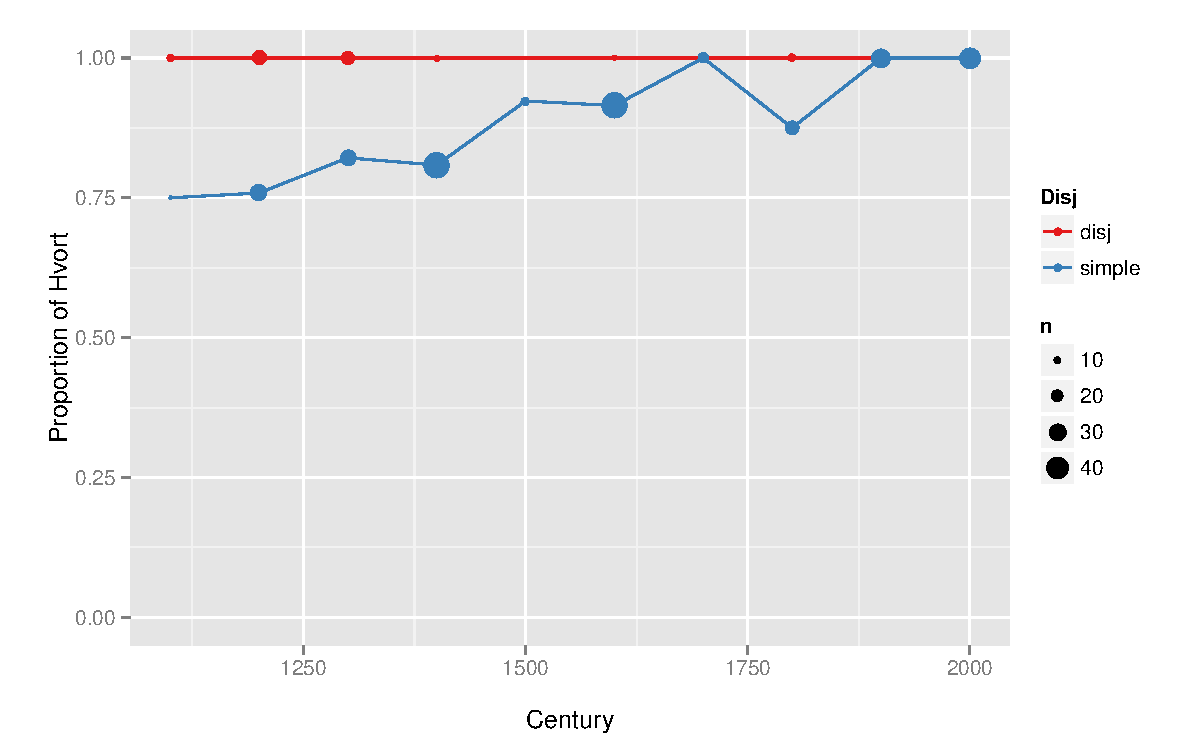
\includegraphics[scale=.7]{whetherifIce.pdf}
    \caption{Replacement in Icelandic of \textsl{ef} (``if'') by \textsl{hvort} (``whether'') in embedded polar questions. N = 397 clauses, IcePaHC. Texts binned by century.}
       \label{hvort}
    \end{center}
\end{figure}

In English, on the other hand, polar questions with \textsl{whether} have specialized slowly over time for the disjunctive context, while \textsl{if} has slowly specialized for polar questions without disjunctions.
The diachronic trend in English is shown in Figure \ref{whetherfig}.

\begin{figure}
    \begin{center}
    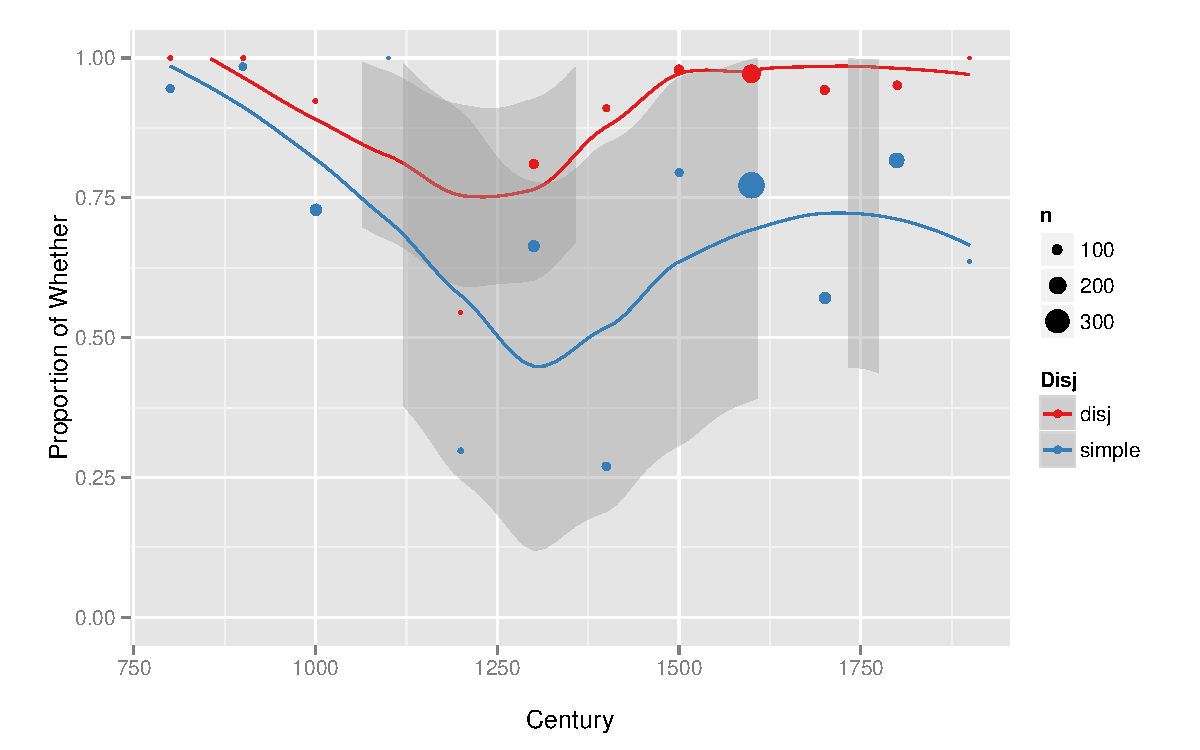
\includegraphics[scale=.7]{whetherifEngLoess.pdf}
    \caption{Specialization in English of \textsl{if} and \textsl{whether} in embedded polar questions. N = 1929 clauses; corpora: IcePaHC. Texts binner by century, and loess curve shown (due to the considerable noise in parts of the sample).}
    \label{whetherfig}
    \end{center}
\end{figure}

Figure \ref{whetherfig} shows the two variants slowly diverging in their favoring contexts, so that \textsl{whether} is favored more and more over time by the disjunction context, while the simple context comes to increasingly favor the \textsl{if} variant.
Though the data is admittedly noisy, no doubt due to imperfect dating and sampling of dialect and genre during the Old and Middle English periods, a statistical model confirms that the diachronic trend is indeed one of specialization. \notejoel{should be a mixed model...oh dear}
This effect is what our theory predicts for competing grammars in the absence of a selective pressure in favor of one of the variants, or in the case where the selective pressure is smaller than the effect of the Principle of Contrast.


\begin{figure}[h!tbp]
	\centering
	\subfloat[][Icelandic\\Replacement]{
	 	\def\svgscale{0.55}
		\import{figures/}{hvort.pdf_tex}
		\label{hvort}
	}
	\qquad
	\subfloat[][English Specialization]{
		\def\svgscale{0.55}
		\import{figures/}{whether.pdf_tex}
		\label{whether}
	}
 \caption{Contrasting the historical development of {\it hvort/ef} and {\it whether/if} in Icelandic and English}
 \label{whether_if_diagram}
\end{figure}

\subsection{Sketch: A Model For Specialization along a Categorical Dimension}
\label{catspec}

This last point requires some elaboration.
Since the Principle of Contrast is a fundamental part of every child's acquisition strategy (as suggested in the acquisition literature), it must be present as a factor in every case of change.
Obviously, if no selective pressure exists driving one member of a doublet to replace the other, then the Principle of Contrast will assert itself.
However, it may be rare for there to be \textsl{no} selective pressure at all in a given case.
Therefore, in cases where selection operates, both selection and the Principle of Contrast affect the situation of competing grammars simultaneously, and they each bleed each other: specialization prevents selection, and selection can prevent specialization.
In order to be precise about how selection and specialization interact, we first sketch a model of how specialization might actually proceed in acquisition, considering the relatively simple case of specialization along a categorical dimension.

Let's being by assuming, for the sake of argument, a simplified model of acquisition along the lines of \citet{yang2000,yang2002}: a child is presented with one piece of data at a time, each of which may contain one of the two variants in the doublet, variant A or variant B, and the child attempts to keep track of the abundance of each variant in the speech community.
They do this by updating, online, frequency estimates for A and B every time they receive a token of one or the other.
We will refer to these frequency estimates as $x_A$ and $x_B$; e.g. $x_A$, at any given point in the learning process, is the proportion of times the child has heard the A variant, and $x_B = 1-x_A$.
From this starting point, we can complicate the scenario by introducing first, a selective pressure, and then, the Principle of Contrast.

One point which is implicit in Yang's model is that the child's tracking of frequencies for A and B, $x_A$ and $x_B$, actually only makes sense if the child is tracking them within some linguistic context, $C$, in which the child knows that either variant can occur without any difference in meaning; indeed, this is the definition of the linguistic variable in the sociolinguistic tradition, beginning with \citep{wlh1968}.
\footnote{For the purposes of the illustration, this could be a semantic, grammatical, or sociolinguistic context; it is any context for which children can theoretically specialize linguistic variants.}
(Alternatively, we might assume that the child track's the variation in all possible contexts simultaneouly, i.e. for $C$ where $C$ is any context where the variants may occur, but this is simply a special case of the general model we are describing.)
So we assume that the child listens for A and B in Context $C$, which must be some context in which the child can reasonably expect to hear either A or B variants.
(Note that every doublet has this property, with respect to some context, at the point in history just after it is innovated; at that point, no specialization has occurred yet.)
We can now introduce a selective pressure in favor of variant B, of the following type:
if a given piece of data contains variant A, there is some probability $p$ that the child will not be able to process the variant and will therefore merely treat it as noise; it does not ``count'' for the child's memory of how many times they've heard the variant.\footnote{The advantage could actually be due to any cause, not just processing, but I use processing as a fairly simple example of a possible issue that might lead to a selectional pressure.}
Over time, this will lead to the child systematically overestimating the frequency of B in the input, as there is a bias in favor of updating $x_B$ that does not exist for $x_A$.
(This gives variant B a selectional advantage of $1-p$ over A.)

The Principle of Contrast comes into the acquisition process when the child decides to change the selection dynamics, by actively privileging one of the variants in a particular context, which we might refer to as $C_i$ (where $C_i$ is only one out of many possible contexts where the variation shows itself, $C_1$...$C_n$).
We will refer to this process as \textbf{assignment}, and the diachronic specialization of variants for different contexts is the result of iterative \textbf{assignment} during acquisition, and during generations of acquisition.
To see how this works, consider the situation we mentioned above, where variant B is replacing A in all contexts, all in lockstep with each other; in this case, the child only needs to keep track of a global $x_A$ and $x_B$, which will be the same in every context.
We can then think of assignment as the child taking the following two steps: first, they decide to decouple the variants' probability estimates in context $C_i$ from those for the rest of the contexts and keep track of $x_{A_{C_i}}$ and $x_{B_{C_i}}$ separately from the others (i.e. separately from $x_{A_{C_{i+1}}}$...$x_{A_{C_{n}}}$, etc.).
Secondly, once the first step is done, the child decides to specifically associate one of the variants with $C_i$, privileging that variant by augmenting its probability estimate \textsl{for that specific context alone}, above and beyond whatever global process of selection may already be taking place across all contexts.
For example, encountering a piece of A data in $C_i$, the child might double-count it in calculating $x_{A_{C_i}}$, which is of course a probability estimate that is only relevant to $C_i$.
(Alternatively, the child could encounter a piece of B data in $C_i$, and ignore it completely, which would have the same effect of bumping up $x_{A_{C_i}}$.)
This adds to the system a selective pressure in favor of A, but one that \textsl{only} applies in $C_i$.
If the child thus assigns A to $C_i$ at the same time as there is a global selective pressure in favor of B, then as these processes iterate over time, A will become specialized for $C_i$ as B beats out A in all other contexts; in effect, this is equivalent to B becoming specialized for $C_{i+1}$...$C_n$.
This is a rather nice result, in fact, as we have now reduced specialization to a special case of selection: context-sensitive selection, with the Principle of Contrast being a type of selective pressure.

Of course, in the case above specialization only results if the rate of assignment is rapid enough (i.e. the selective pressure in $C_i$ is strong enough) for A to replace B in $C_i$ before the global selective pressure in favor of B causes B to replace A everywhere, including $C_i$.
In other words, the local selective pressure of assignment for A in context $C_i$ must be greater than the global selective pressure in favor of B, so that there is a net selective pressure in favor of A just in the context $C_i$.

%Suppose the Principle of Contrast causes the child to assign a token of A, whichever they happen to hear, to context $C$ (i.e. beginning to specialize it for that context, adding a selective pressure in that context only in favor of A) with probability $q$ in the absence of any interfering selective pressure.


%Note that since the Principle of Contrast is about \textsl{contrasting} variants, if the child is presented with a token of B, for example, and assigns the token of B to context $C$, then we assume they simultaneously assign a (hypothetical) token of A to context $not-C$.
%Note also that assignment does not mean that the entire category of B is assigned to context $C$ just because a single token has been assigned; assignment of B to $C$ means that the child keeps an online estimate of their confidence that category B is specialized for $C$, and the child updates this measure of confidence a little at a time.
%This is also why, if the child assigns a token of B, it is possible for her to simultaneously assign a ``token'' of A, even though they haven't encountered a real token of A on that round of acquisition; we simply mean that the measures of confidence for both B and A are updated simultaneously.

\subsubsection{A little more mathematical detail}

At this point, we can explore, in a little more detail, how assignment (i.e. context-dependent selection) might interact with a global selective pressure.
Continuing our hypothetical situation above, in which B has a global selectional advantage over A, suppose that in context $C_i$ only, the child ignores tokens of B with a probability $q$, perhaps treating $q$ proportion of B tokens as noise in that context.
Now we have a global selectional advantage for B which operates in all contexts (i.e. the child mishears A with probability $p$), and in addition, a local selectional advantage for A which only operates in context $C_i$.
So, if an A token is uttered in $C_i$, the probability of the child counting it is $(1-p)$, and if a B token is uttered, the probability of the child counting it is $(1-q)$.
The rate of specialization of A in $C_i$ can be represented as $(1-p) - (1-q)$; this is the difference between the local advantage of A and the global advantage of B.
B will continue to replace A in other contexts at a rate of $(1-q)$
If $(1-p) - (1-q) > 0$, then specialization takes place at this rate; if not, then the difference between the advantages is a measure of how the replacement of A by B is slowed in context $C_i$.

%if the child hears a token of B, they will assign B to a specific context with probability $q$; the probability of assignment for B is just the overall probability of assignment, since B is not disadvantaged in any way.
%However, if the child hears a token of A, they will fail to hear it $p$ amount of the time, and so if A is presented to the child, they will only successfully assign A (and B) to the current context (and B to its complement) with probability $(1-p)q$.
%Clearly, as the selectional advantage increases, the rate of specialization will slow, as the probability for assignment any given token will decrease.
%The overall probability of assignment in context $C$ will then be a function of the probabilities above, and the actual abundances of variants A and B for context $C$ in the input.
%If variants A and B occur $a$ and $b$ proportions of the time in context $C$ (i.e. occur with probabilities $a$ and $b$ in that context), then the overall probability of assignment of some arbitrary variant, given that context will be: $(1-p)aq + bq$

%(Of course, any progress on specializing the variants in a given generation will affect the abundances of the two variants in each context for the next generation.)


However, if the selectional advantage of one variant over another is small enough that the speed of selection is slower than the speed of specialization, specialization should eventually win out and ultimately remove the selective process (asssuming a case where specialization can go to completion).
This is because the competition between the variants can only occur when they mean the same thing and can occur in the same context; as they specialize, they are no longer competing for the same resources, for the same context in the speaker's use.
In fact, we can add something to our theory of this race between selection and specialization: while selective advantage can be of various sizes, since the Principle of Contrast is a fundamental property of the cognitive system responsible for acquisition, it should really be constant across individuals (modulo expected variation in brain structure).
Hopefully, by investigating the cases where specialization is able to go to completion and comparing them to those where selection goes to completion, we may eventually be able to calculate the constant rate of specialization.


\subsection{A model of specialization along a continuous dimension}

So far in this section, we have illustrated the first two scenarios (from the end of section \ref{options}) for the diachronic evolution of doublets, and provided the beginnings of a formal model for them: replacement changes and specialization along a categorical dimension.
Both of these changes have the potential to go entirely to completion given enough time, where ``completion'' means that the probabilistic variation between two (or more) forms ultimately ceases to exist.
As we've said above, the probabilistic variation can either cease to exist because one form disappears completely (i.e. replacement has gone to completion) or because the two forms end up in totally complementary distribution (i.e. specialization has gone to completion along a categorical dimension).
At this point, we must consider the third scenario from section \ref{options}: specialization of categorical variation along a continuous dimension.
This type of specialization simply cannot go to completion, in the sense above, but significant partial specialization can take place.


As a proof of concept for this idea, we built a computational model of the acquisition and generational transmission of sociolinguistic variation which encodes only the simplest and most empirically motivated assumptions about how assignment might proceed in acquisition.
The results of the simulation below show that categorical variation can indeed specialize along a continuous dimension in a way that results in diachronic stability (or near stability), even when no direct pressure to specialize is encoded in the model.
The model allows the hypothetical learner to assign (i.e. specialize) the variants, by allowing them to take different values along the continuous dimension, but it does not enforce specialization.

Consider the case in which a child specializes \textsl{-in}/\textsl{-ing} along the continuous dimension of style.
Unlike the specialization along a categorical dimention above, the context $C$, to which a learner can assign one of the two variants, can be any value along a continuous scale of style.
For the purposes of this illustration, possible values of $C$ (i.e. possible speech style contexts) will be all real numbers from 0 to 100, where 0 is most colloquial and 100 is most formal.
\footnote{Of course, in reality there may not be endpoints to a style scale; it could easily be the case that style-shifting can take arbitrarily formal or colloquial values, depending only on the structure of the society in which the speaker lives.}
The learner in the simulation listens to a speaker speaking in a particular style, a particular numerical value of $C$, and the value of $C$ is assumed to be shared information between the speaker and learner (e.g. we assume the child has learned the relevant social cues, which must happen very early, as shown in e.g. \citealt{smithetal2007}).
As the learner hears the speaker use one of the variants in style $C$, they try to use $C$ to determine a mean style value for when the variant should be used.

The simulation proceeds as follows:

\begin{itemize}
		\item[ ]\textbf{Generation 0:}\\  -\textipa{In}$\sim$-\textipa{IN} doublet is innovated, with no stylistic conditioning. \textbf{Gen 0} picks a style to speak in (by pure chance), and produces a variant, repeats. 
		\item[ ]\textbf{Generation 1:}\\  \textbf{Gen 1} learns an estimate for the (mean) style value of -\textipa{In}, \textipa{IN}, as soon as they hear the first tokens of each from \textbf{Gen 0}. She adjusts this estimate as they get more data from \textbf{Gen 0}.\footnote{The size of the adjustment, and hence the posterior value for the current variable's mean style estimate, is a function of the prior estimate, and the distance between the current style and the prior style. For details, see the simulation script in \texttt{github.com/joelcw/tyneside/blob/master/articles/sim\_Gauss.R}}
		\item[ ]\textbf{Generation 2:}\\ \textbf{Gen 1} picks a style, chooses one of the variants to produce with a probability weighted by how far their style estimates are from the current style,\footnote{The probabilities are derived from assuming that each variant has a Gaussian probability density function over styles, with the mean of the distribution being the speaker's current mean style value estimate for the variant. Again, for details, see script in \texttt{github.com/joelcw/tyneside/blob/master/articles/sim\_Gauss.R}} and repeats. \textbf{Gen 2} learns style estimates for variants as above.
		\item[ ]\textbf{Repeat...}
\end{itemize}

%todo: the next few sentences will have to be revised if we change the def of assignment above to exclude "not-C"
Note that the algorithm above is a very simple model of the acquisition process.
First, the learner does not store every token; they just keep one estimate for each variant of the mean style that the variant should be associated with, so only one number for each variant is carried forward as the algorithm iterates.
Another way in which this model for specialization along a continuous dimension is different from the case of categorical specialization in section (\ref{catspec}) is the following: the assignment of a mean style value to one variant does not also result in the assignment of a ``$not-C$'' mean style to the other variant.
As the dimension is continuous, which means each variant has a probability distribution over contexts with a certain mean, ``$not-C$'' is not really a definable context.
For now, we assume this means that the child does the maximally simple task: update the mean style estimate for the given variant, and do nothing to the mean style estimate for the other variant.
This is an important point: the Principle of Contrast in not hard-coded in the algorithm at all; the learner has the possibility of keeping the estimated mean style values distinct for the two variants, but no requirement that they be distinct.
As you will see below, the Principle of Contrast simply emerges by iterating the algorithm over generations.

Running this model over 20 generations produces the chart below.




 %state what assumptions are not there

%This actually implies that speakers could theoretically map continuous linguistic variants on to continuous social dimensions, possibly

%3 Important take-away points from the simulation:

%1) We didn't build the Principle of Contrast into the model
%2) The variants do specialize, but not all the way to the limits -- they stabilize at the quartiles
%3) The specialization stabilizes at 20000 tokens, but with 1000 tokens it never does. This implies that the frequency of the variant could be a determining factor
%of whether the variation results in specialization or replacement. (If the simulation is initialized by the first variants the adult utters -- this is important, because it is one *less* assumption in the model, i.e. there is no default value.)

\section{Case Studies}
\label{cases}

%Should this section really be here at all? Or just to show the continuous dimension. If so, then forward reference above.
\subsection{Topicalization (English Object Fronting)}
\label{topsect}


\subsection{\textsl{-in}/\textsl{-ing} Variation}
\notejoel{Do we really want to use this? Do we really want t/d also?
We could stay away from these since they seem to be a mix of lexical and morophological.
Instead, could use:}

\subsection{\textsl{h}-Dropping}

Baranowsky \& Turton (\textsl{to appear}) \notejoel{get ref} present a quantitative study of syllable-initial [h]-deletion in Manchester, which illustrates our theory of (apparent) stable variation in the phonological domain: two categorical variants have partially specialized along a continuous extragrammatical dimension.
``\textsl{h}-dropping'' is characterized by the presence or absence of initial [h] in the relevant set of words, and is clearly a case of categorical variation in the phonological domain, so it is a candidate for the kind of specialization we have described above.
The variation is definitely phonological in nature, rather than purely phonetic (i.e. either a new allophone of /h/, or total loss of the phoneme /h/ in the relevant positions), as can be seen from its interaction with the phonological rule of [\textipa{\*r}]-insertion (``linking'' \textsl{r}):




	\begin{exe}
		\ex \quad \textsl{Harpurhey}
		\begin{xlist}
			\ex \label{har1} $[$\textipa{""ha:p@"heI}$]$
			\ex \label{har2} $[$\textipa{""a:p@"\*reI}$]$
		\end{xlist}
	\end{exe}

\noindent (\ref{har1}) is the variant with [h]s intact, while (\ref{har2}) shows two deletions (or absences) of [h].
The absence of [h] in syllable-initial position of the final, stressed syllable in (\ref{har2}) triggers application of the intervocalic [\textipa{\*r}]-insertion rule, and so [\textipa{\*r}] appears in the onset of that syllable on the surface.
	
Baranowsky \& Turton (\textsl{to appear}) show that while \textsl{h}-dropping is variable, it is remarkably stable across an apparent time distribution in that speech community.
This is unlike the other phonological processes they investigated, ``t-glottaling'' and ``th-fronting'', which are subject to various sociolinguistic factors, but nevertheless show a change in progress across the ages in the sample.
%Furthermore, as the deletion of [h] (or realization of /h/ as 0) occurs both at the beginning of words and word-internally in syllable-initial position (e.g. \textsl{behind}), the phenomenon is most likely a phonological rule.

Our theory predicts that the apparent stability of \textsl{h}-dropping should be due to specialization, but as it remains probabilistic, there must be a continuous domain of specialization involved. Baranowsky \& Turton find that style, a continuous social dimension, conditions the \textsl{h}-dropping variation.
According to the theory we have presented, specialization removes the overlap in funtional context which creates the competition between variations, and so the variation can stabilize, rather than going to completion as a replacement change in progress.
Specialization along a continuous dimension means that probabilistic conditioning of the variants still persists, even as the variation comes close to stabilizing over time.

It is important to be careful at this point, however: we are not claiming that specialization along style is sufficient to remove all of the competition and stop the change completely; our theory only states that much or most of the competition can be removed in this way, but at best, the change can only be slowed.
(We discuss this in greater detail in section \ref{relclause} below.)
Indeed, Turton \& Baranowsky also investigate the variation ``\textsl{th}-fronting'', which is both a change in progress and shows specialization of the variation along the style dimension.
In that case, specialization along style may have slowed the change, but it clearly has not stopped the change.
The \textsl{h}-dropping variation, on the other hand, has been slowed to the point where there is no significant change that is observable in apparent time; it appears stable, at least to the limits of our current ability to measure the variation over time (e.g. given a limited time window and noise in the measurements).

So why is \textsl{h}-dropping more stable over time than \textsl{th}-fronting?
The answer probably lies in the fact that the \textsl{h}-dropping variants are actually more specialized that the /th/-fronting variants: \textsl{h}-dropping is also conditioned by the categorical factors of grammatical category and preceding pause, in addition to style.
It is likely that the three-way specialization has removed much more of the competition in the \textsl{h}-dropping case than has been removed in the /th/-fronting case, which only shows two-way specialization (style and following segment).
In this way, what at first appears to be a challenge to our theory, the fact that \textsl{th}-fronting is not as stable as \textsl{h}-dropping, actually turns out to be nicely explained by our theory: more simultaneous domains of specialization means more specialization, less competition, and greater stability over time.

But even if the combination of continuous and categorical domains of specialization is important for the overall stability of \textsl{h}-dropping, it is the presence of a continuous domain of specialization, style, which allows the variation to remain stochastic, even while it is stable in the apparent time window that Turton \& Baranowsky were able to observe.


\subsection{Relative Clause Extraposition}
\label{relclause}
%agnostic as the rightward/leftward-movement question
%Cite Anton about phonological weight being continuous, not discrete !!!

\subsection{t/d Deletion}
%greg guy, joe's stuff
%Ricardo's work




\section{A Related Case: Phonetic Implementation of Phonological Categories}


\section{Predictions of the Theory (or an Invitation to Falsification)}
BIG POINT: comparing two different variables, two different changes is very complex because of the number of different possible dimensions of specialization, and other factors like the absolute frequency (rarity) of the variable.
So the best test is the same variable in two different populations, like the \textsl{whether/if} study.

\subsection{Style and Third-Wave Sociolinguistics}



%talk about how the specialization should happen in detail along the continuous dimension
%Actually, one prediction is that the Principle of Contrast and Darwinian selection should operate simultaneously: the variants should begin to specialise even as one is taking over the other's function...the question is whether they can specialize fast enough to beat the selection. Of course, if there is no selective pressure at all (or a sufficiently weak one), then the specialization can proceed at whatever leisurely pace it wants (this seems to be the case for English ``whether''). So for changes that go to completion, there should still be evidence of some earlier specialization.


\subsection{Dative Shift}

\subsection{Particle Shift}
%Dehé


According to our theory, it is also possible for these same cases of variation to result in specialization in some speech communities, but for one variant to replace the other in other speech communities.
%t/d in AAVE (get refs)
%in/ing in Ulster Scots (get refs) / scottish english - see Miriam Meyerhoff's recent paper on Poles in Edinburgh, and thank Lauren

%extraposition in modern Dutch and German, which has specialized along a grammatical, categorical dimension
\section{Conclusions}

%The information structural criteria are categorical, but probably not the phonological conditioning 

%Cite Anton about phonological weight being continuous, not discrete !!! Also, Laurel on subject-length

%Cite Laurel's thesis about model of use, and subject length

%Cite Japanese Honorific variation -- thank Caroline -- Anna Strycharz

%t/d in style-shifting -- Jen Smith paper and refs

Figure \ref{competition_figure} sums up the possible outcomes of competing forms A and B that we propose. 
At the onset, a new linguistic form, B, is introduced to the linguistic inventory.
How and why such an event occurs is well outside the scope of this paper, and attempts in the field to resolve this Actuation Problem are active.







% For one-column wide figures use
%\begin{figure}
% Use the relevant command to insert your figure file.
% For example, with the graphicx package use
%  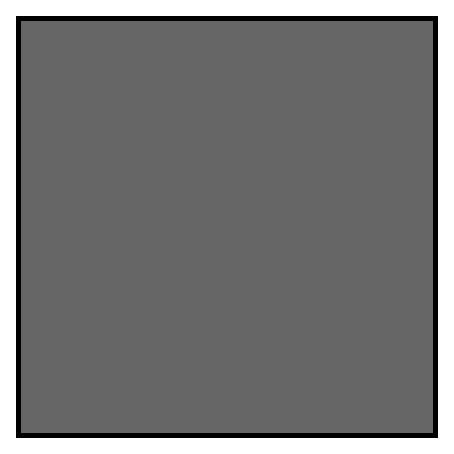
\includegraphics{example.eps}
% figure caption is below the figure
%\caption{Please write your figure caption here}
%\label{fig:1}       % Give a unique label
%\end{figure}
%
% For two-column wide figures use
%\begin{figure*}
% Use the relevant command to insert your figure file.
% For example, with the graphicx package use
%  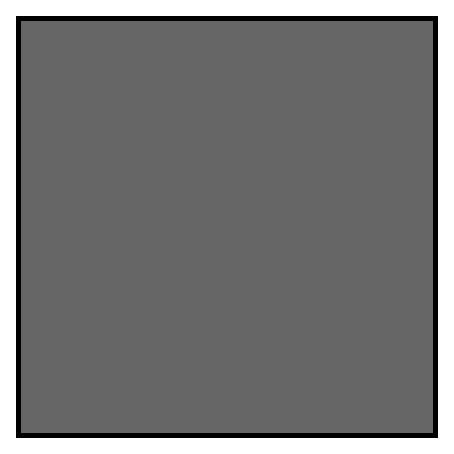
\includegraphics[width=0.75\textwidth]{example.eps}
% figure caption is below the figure
%\caption{Please write your figure caption here}
%\label{fig:2}       % Give a unique label
%\end{figure*}
%
% For tables use
%\begin{table}
% table caption is above the table
%\caption{Please write your table caption here}
%\label{tab:1}       % Give a unique label
% For LaTeX tables use
%\begin{tabular}{lll}
%\hline\noalign{\smallskip}
%first & second & third  \\
%\noalign{\smallskip}\hline\noalign{\smallskip}
%number & number & number \\
%number & number & number \\
%\noalign{\smallskip}\hline
%\end{tabular}
%\end{table}


%\begin{acknowledgements}

%\end{acknowledgements}

% BibTeX users please use one of
%\bibliographystyle{spbasic}      % basic style, author-year citations
%\bibliographystyle{spmpsci}      % mathematics and physical sciences
%\bibliographystyle{spphys}       % APS-like style for physics
\bibliographystyle{linquiry2} %use spbasic for journal of comparative gmc linguistics, etc.
\bibliography{joelrefs}   % name your BibTeX data base

\end{document}
% end of file template.tex

 